\documentclass[t]{beamer}
\usepackage{beamerthemesplit}
\usepackage{xcolor}
\usepackage{color}
\usepackage{colortbl}
\usepackage{tikz}
\usepackage{epsfig}
\usepackage{epstopdf}
\usepackage{subfigure}
\usepackage[absolute,overlay]{textpos}
\usetheme{USC}

\tikzset{
  every overlay node/.style={
    draw=none,fill=none,rounded corners,anchor=north west,
  },
}
% Usage:
% \tikzoverlay at (-1cm,-5cm) {content};
% or
% \tikzoverlay[text width=5cm] at (-1cm,-5cm) {content};
\def\tikzoverlay{%
   \tikz[baseline,overlay]\node[every overlay node]
}%

\definecolor{pathgreen}{RGB}{2, 155, 81}
\definecolor{pathblue}{RGB}{0, 124, 181}

\usepackage{amsmath}
\usepackage{mathtools}
\DeclareMathOperator*{\argmax}{arg\,max}

% Table
\usepackage{multirow}
\usepackage{colortbl}
\definecolor{kugray5}{RGB}{224,224,224}
\usepackage{rotating}

\begin{document}

\graphicspath{ {Graphics/} }

\title[USC Viterbi School of Engineering]{An On-line Truthful and Individually Rational Pricing Mechanism for Ride-sharing}  
\author[Mohammad Asghari]{\small{Speaker:}\\Mohammad Asghari\\
\vspace{0.05in}
\begin{flushleft}
\tiny{
\hspace{1.25in}Joint work with\\
\hspace{1.25in}Cyrus Shahabi, Faculty of Computer Science at University of Southern California}\\
\vspace{-0.25in}
\end{flushleft}}

\date{Nov 8, 2017} 
\begin{frame}
\titlepage
\vspace{-0.5in}
\begin{columns}
  \column{.2\textwidth}
  \begin{center}
    
\includegraphics[height=1.5cm]{viterbi_logo.jpg}
  \end{center}
  \column{.6\textwidth}
  \column{.2\textwidth}
  \begin{center}
    
\includegraphics[height=1.5cm]{imsc_logo.jpg}   
  \end{center}
\end{columns} 
\end{frame}

\section*{Introduction}
\begin{frame}\frametitle{Motivation}
\begin{figure}
	\centering
    
\includegraphics[width = 0.75\columnwidth]{carpool}
\end{figure}
\begin{itemize}
\item<2-> Increasing popularity of commercial ride-sharing platforms
\begin{figure}
	\centering
    
\includegraphics[width = 0.55\columnwidth]{ride-sharings}
\end{figure}
\end{itemize}
\end{frame}

\begin{frame}\frametitle{Motivation}
\vspace{-0.28in}
\begin{figure}
	\centering
    
\includegraphics[width = 0.55\columnwidth]{ride-sharings}
\end{figure}
\vspace{-0.23in}
\begin{itemize}
\item Monetary Incentives.
\item<2-> Auction-based framework for ride-sharing \textbf{(SIGSPATIAL'16) [1]} 
\vspace{-0.1in}
\only<3->{
\begin{figure}
	\centering
    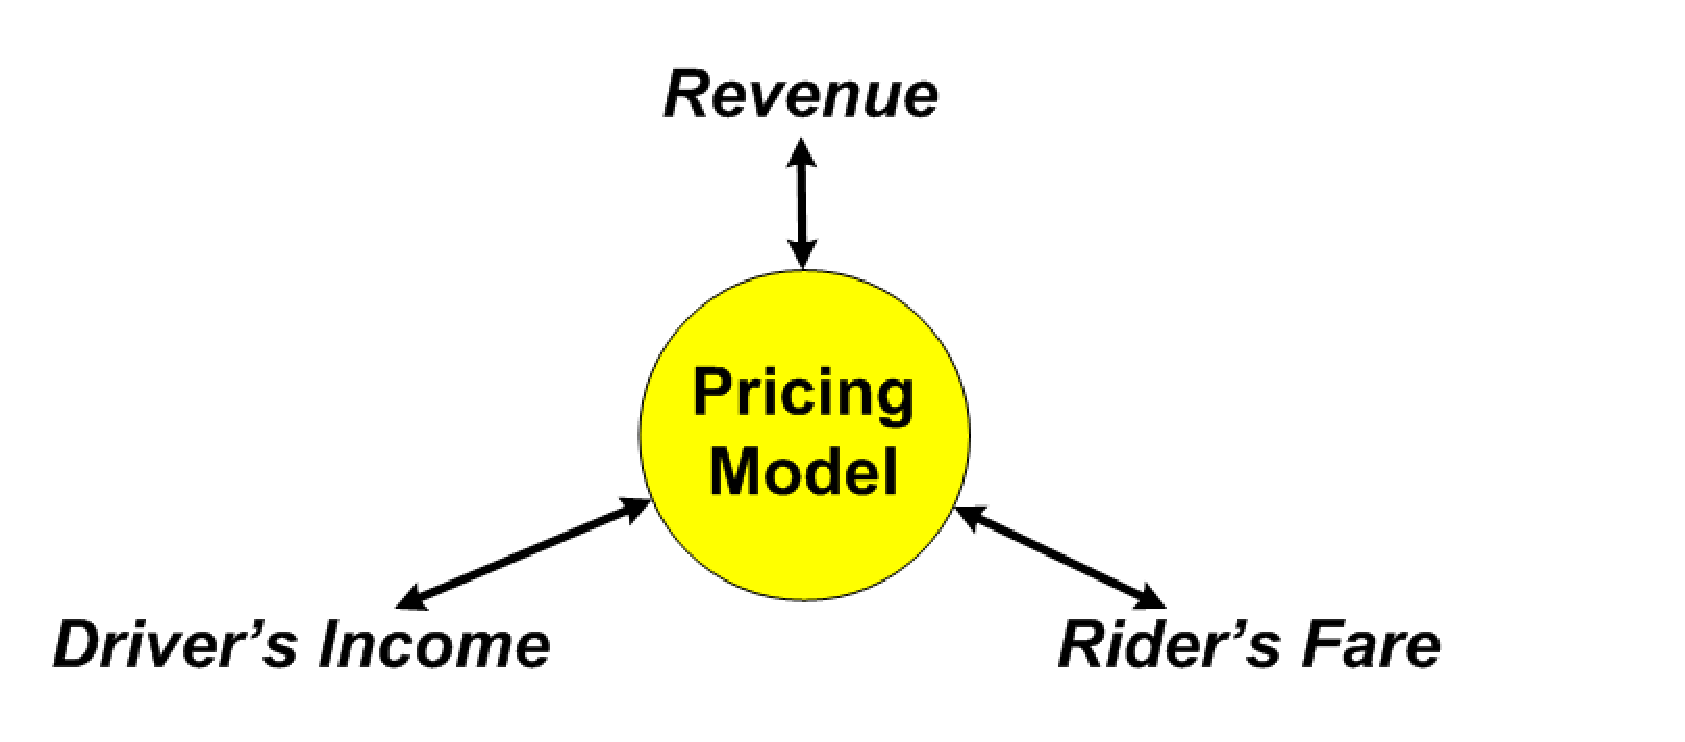
\includegraphics[width = 0.75\columnwidth]{pricing3}
\end{figure}
}
\end{itemize}
\only<3->{
\vspace{0.2in}
\tiny{[1] Asghari et. al., Price-aware Real-time Ride-sharing at Scale - An Auction-based Approach, SIGSPATIAL'16, San Francisco, CA}
}
\only<4>{
\begin{textblock*}{7cm}(3cm,4.5cm)
\begin{block}{}
\begin{itemize}
\item \large{\textbf{Can the drivers cheat?}}
\item \large{\textbf{How can we prevent it without sacrificing revenue?}}
\end{itemize}

\end{block}
\end{textblock*}
}
\end{frame}

\section{Framework Overview}
\begin{frame}\frametitle{Overview}
\only<1>{
\vspace{-0.15in}
\begin{figure}
	\centering
    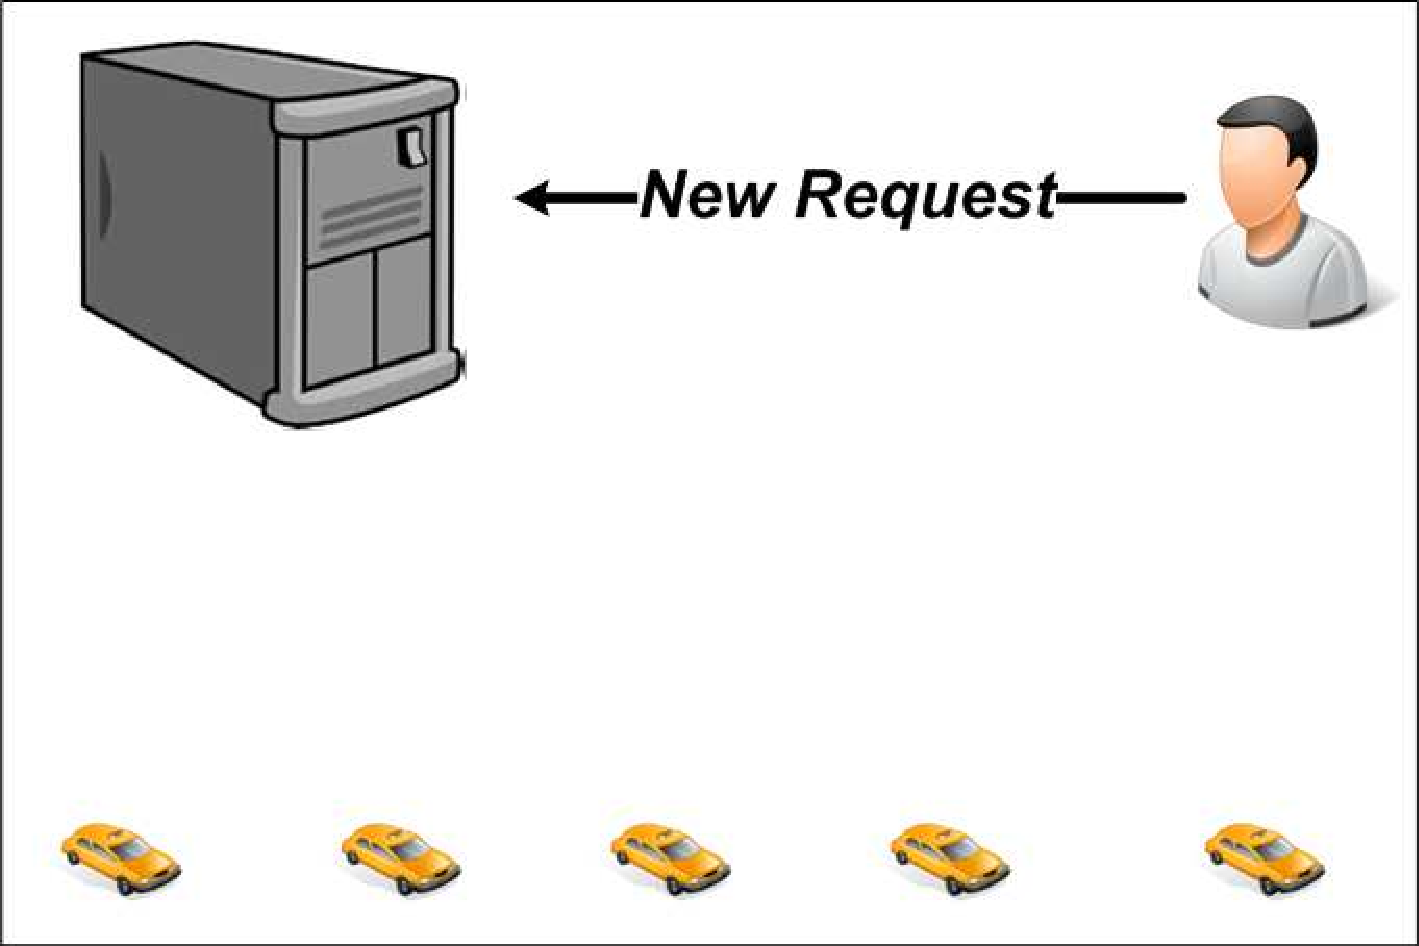
\includegraphics[width = 0.95\columnwidth]{overview1}
\end{figure}
}
\only<2>{
\vspace{-0.15in}
\begin{figure}
	\centering
    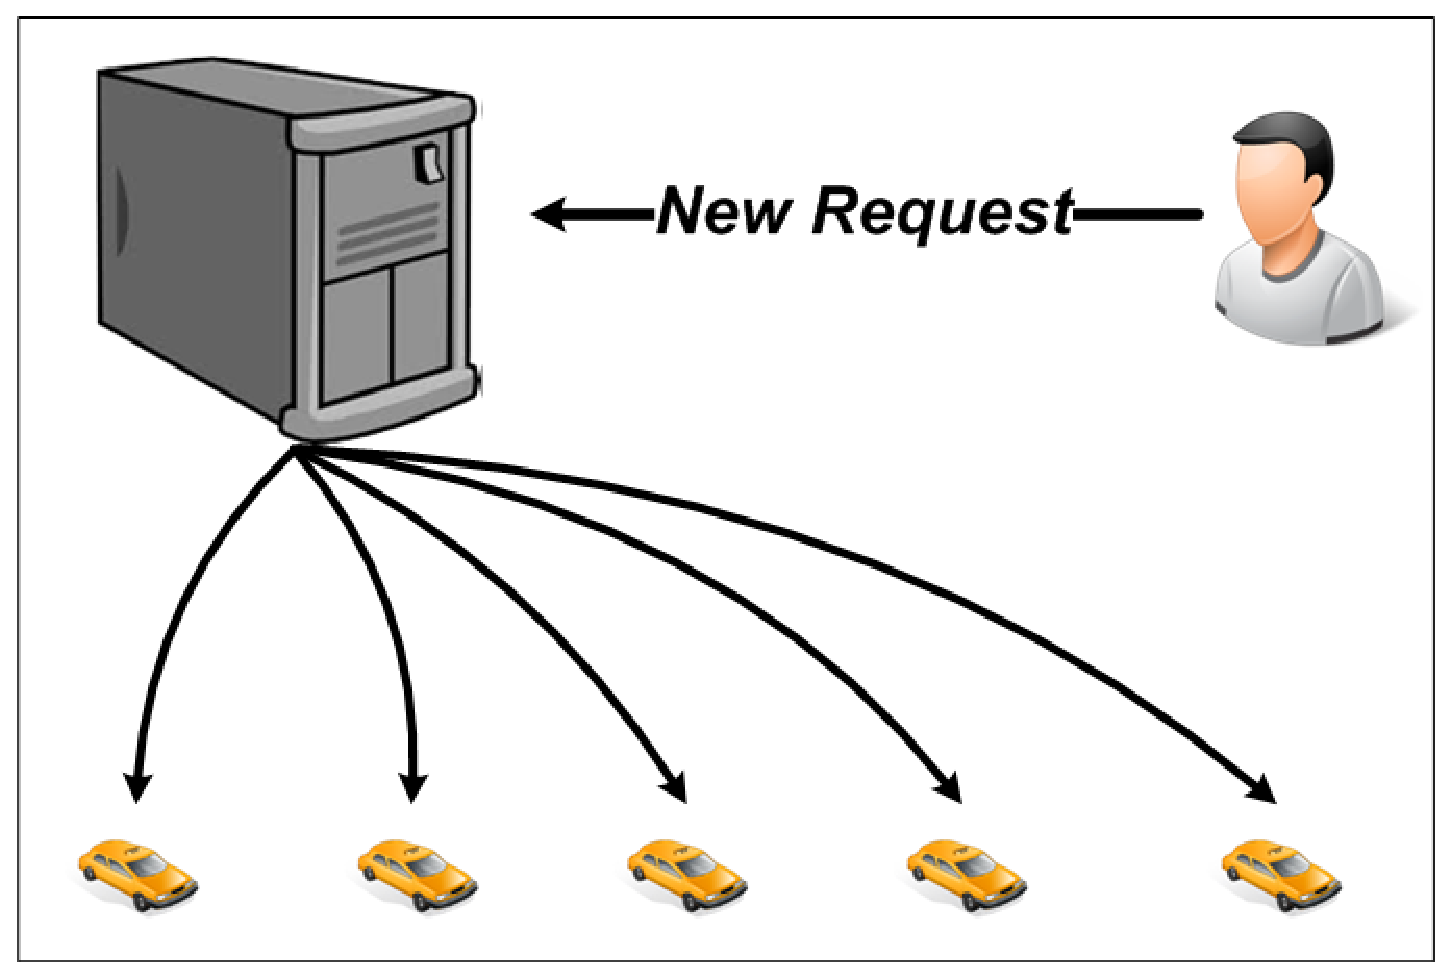
\includegraphics[width = 0.95\columnwidth]{overview2}
\end{figure}
}
\only<3>{
\vspace{-0.15in}
\begin{figure}
	\centering
    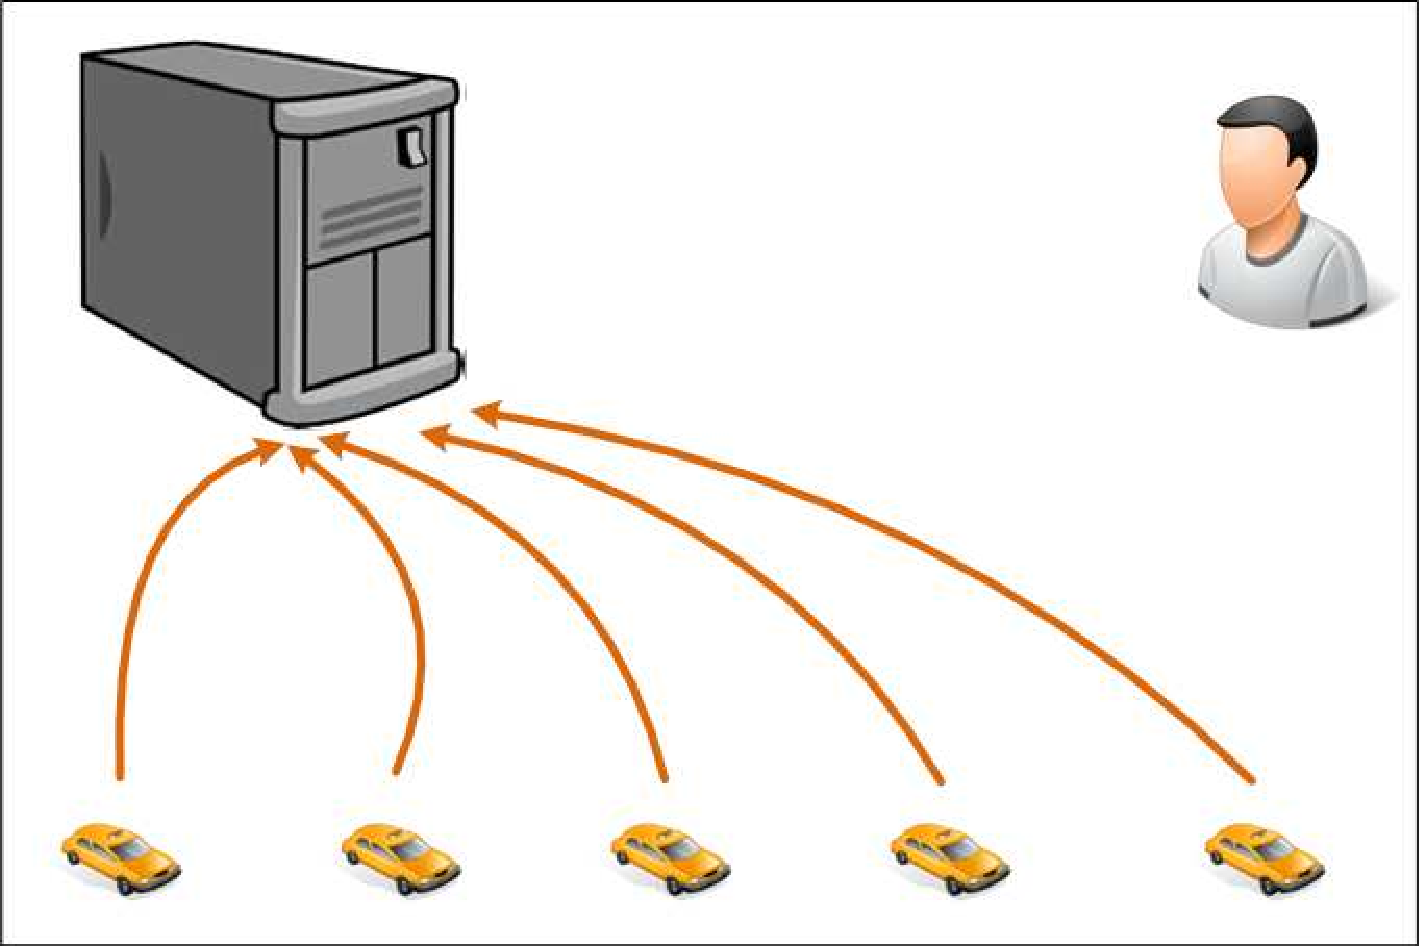
\includegraphics[width = 0.95\columnwidth]{overview3}
\end{figure}
}
\only<4>{
\vspace{-0.15in}
\begin{figure}
	\centering
    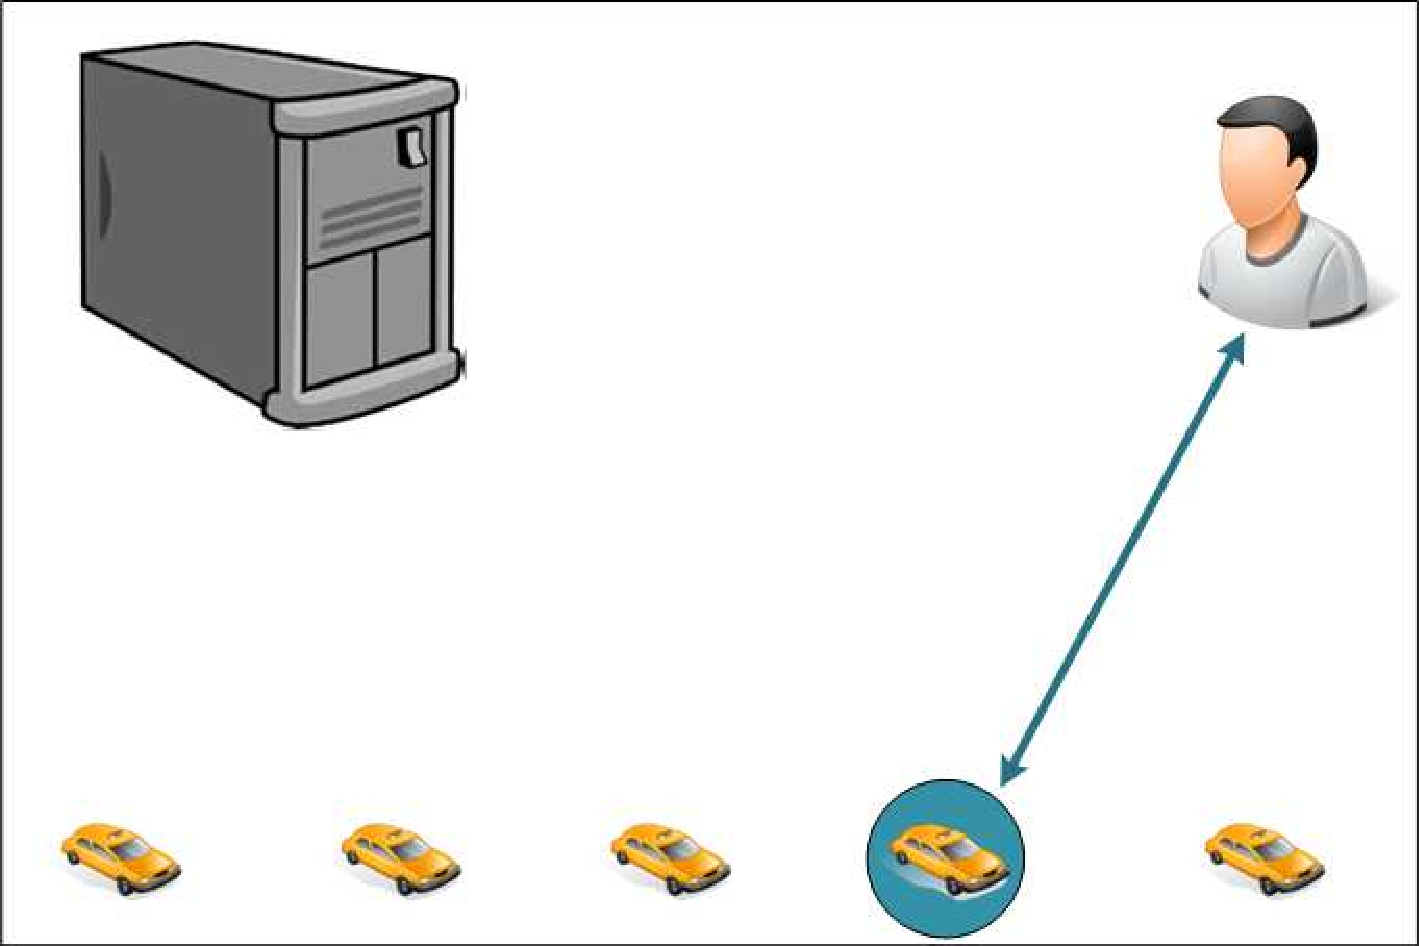
\includegraphics[width = 0.95\columnwidth]{overview4}
\end{figure}
}
\end{frame}

\begin{frame}\frametitle{Bid Computation}
\begin{columns}
\column{0.5\textwidth}
\vspace{-0.3in}
\only<1-2>{
\vspace{-0.15in}
\begin{figure}
	\centering
    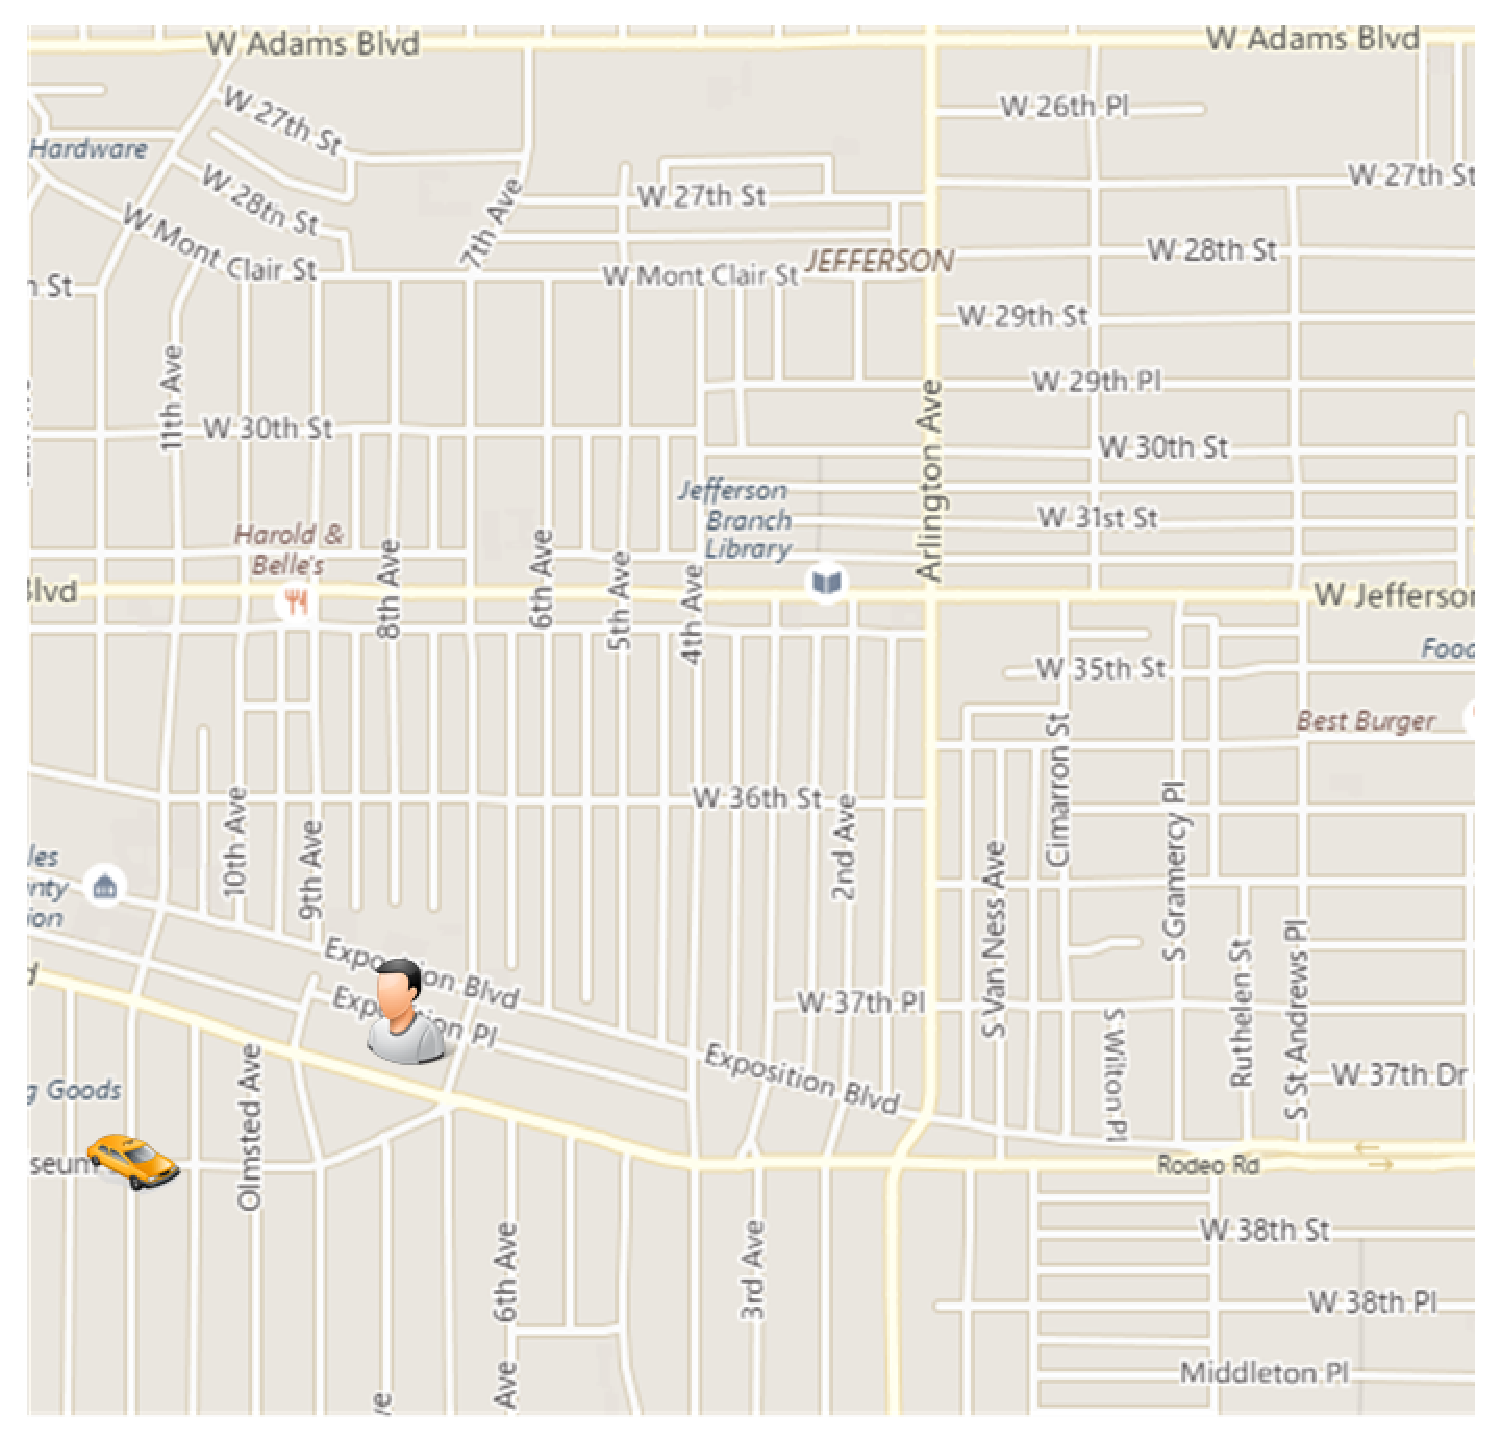
\includegraphics[width = \columnwidth]{bid1}
\end{figure}
}
\only<3->{
\vspace{-0.15in}
\begin{figure}
	\centering
    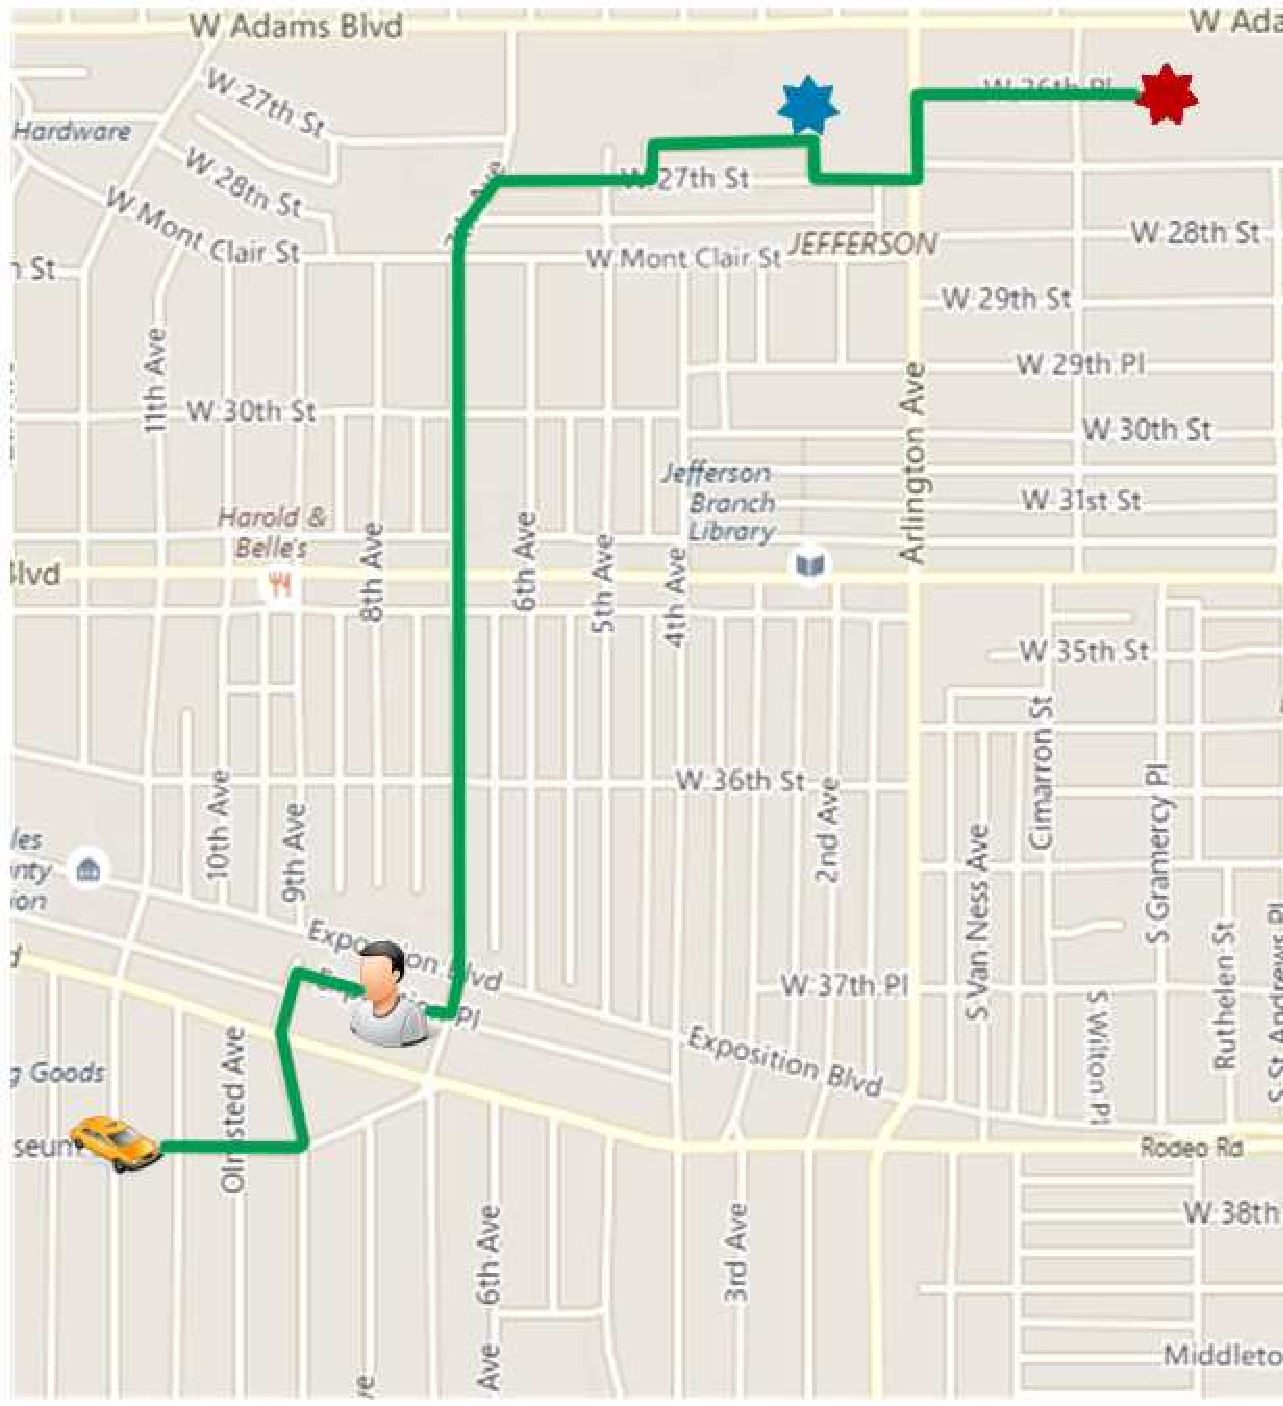
\includegraphics[width = \columnwidth]{bid2}
\end{figure}
}
\column{0.5\textwidth}
\only<1->{
\small{Each driver has a \textcolor{pathblue}{current} schedule $\pi$.}
}
\only<2->{
\small{\begin{equation*}
profit(\pi, \hat{\theta_d)} = \sum_{r \in \pi} fare(r) - cost(\pi, \hat{\theta_d})
\end{equation*}}
}
\only<3->{
\small{For a new request, each driver computes a \textcolor{pathgreen}{best potential} schedule $\pi^*$.}
}
\only<4->{
\small{\begin{equation*}
bid = profit(\pi^*, \hat{\theta_d)} - profit(\pi, \hat{\theta_d)}
\end{equation*}}
}
\only<5->{
\begin{exampleblock}{}
The driver can manipulate his bid by misreporting his type $\theta$.
\end{exampleblock}
}
\end{columns}
\end{frame}

\section{Competitive Bidding}
\begin{frame}\frametitle{Competitive Bidding}
\begin{itemize}
\item Assume the \textbf{true} profit a driver can generate for a request is \$10 but he only bids \$8.
\item<2-> \textbf{If the driver wins}, then he gains an additional \$2.
\item<3-> The \textbf{utility gain} of the driver can be computed as:
\only<3>{
\begin{equation*}
E[u_i] = \left(v_i - b_i \right) \cdot Prob \left[win(b_i)\right] 
\end{equation*}
\begin{itemize}
\item $v_i$ is driver $i$'s \emph{true} valuation (/bid) for the request
\item $b_i$ is what the driver actually bid
\item $Prob\left[win(b_i)\right]$ is the probability that driver $i$ wins the auction by bidding $b_i$.
\end{itemize}
}
\only<4>{
\begin{equation*}
E[u_i] = \left(v_i - \textcolor{red}{s_i\left( v_i \right)} \right) \cdot Prob \left[win(\textcolor{red}{s_i\left( v_i \right)})\right] 
\end{equation*}
\item Our goal is to find a \textbf{strategy function} $s_i(.)$ that any driver can apply to it's \textbf{true} valuation to get his optimal bid.
\begin{equation*}
b_i = s_i(v_i)
\end{equation*}
}
\end{itemize}
\end{frame}

\begin{frame}\frametitle{Competitive Bidding}
\only<1>{
The optimal strategy function can be computed as:
\begin{equation*}
s_i^\prime\left(v_i\right) = \left(n-1\right)\left(\frac{f\left(v_i\right)\,\left(v_i - s_i\left(v_i\right)\right)}{F\left(v_i\right)}\right)
\end{equation*}
\begin{itemize}
\item $n$ is the total number of bidders\\ \textcolor{white}{Propose a Latent Space Transition Model to predict $n$}
\item $f(.)$ and $F(.)$ are the pdf and cdf of the bids\\ \textcolor{white}{We assume $f(.)$ is uniformly distributed in $[0, F(\phi_r)]$}
\end{itemize}
}
\only<2>{
The optimal strategy function can be computed as:
\begin{equation*}
s_i^\prime\left(v_i\right) = \left(n-1\right)\left(\frac{f\left(v_i\right)\,\left(v_i - s_i\left(v_i\right)\right)}{F\left(v_i\right)}\right)
\end{equation*}
\begin{itemize}
\item $n$ is the total number of bidders\\ \textcolor{red}{Propose a Latent Space Transition Model to predict $n$}
\item $f(.)$ and $F(.)$ are the pdf and cdf of the bids\\ \textcolor{white}{We assume $f(.)$ is uniformly distributed in $[0, F(\phi_r)]$}
\end{itemize}
%\begin{columns}
%\column{0.3\textwidth}
%\column{0.4\textwidth}
%\begin{block}{}
%\begin{center}
%Drivers can increase their income by 25\%
%\end{center}
%\end{block}
%\column{0.3\textwidth}
%\end{columns}
}
\end{frame}

\section{Latent Space Transition Model}
\begin{frame}\frametitle{Model}
The number of drivers in location $i$ at time $t$, is the sum of:
\begin{itemize}
\item Drivers that enter the platform in location $i$ at time $t$.\only<2>{\textcolor{red}{[2]}}\only<3->{[2]}
\only<3->{\vspace{0.023in}}
\item Drivers that finish a trip in location $i$ at time $t$.
\only<3->{
\begin{itemize}
\item Need to learn the \textbf{network transition} matrix.
\begin{columns}
\column{0.6\textwidth}
\begin{figure}
	\centering
    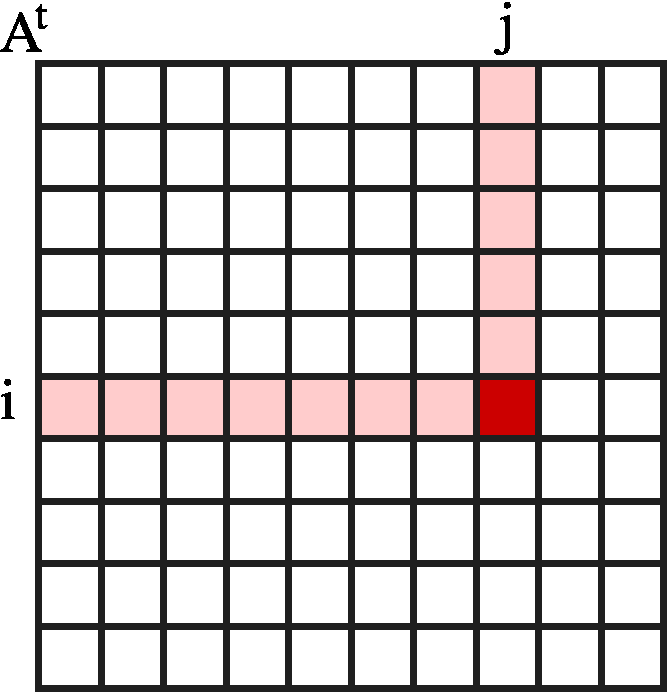
\includegraphics[width = 0.45\textwidth]{network_demand1}
\end{figure}
\column{0.4\textwidth}
\vspace{0.7in}\\
$\alpha_{ij}$ gives the probability of a request with pick-up location $i$ at time $t$ having a destination location $j$.
\end{columns}
\end{itemize}
}
\end{itemize}


\only<2>{
\vspace{2.1in}
\tiny{\textcolor{red}{[2] Cheng et. al., Where are the passengers? A grid-based gaussian mixture model for taxi bookings, SIGSPATIAL'15}}
}
\only<3->{
\vspace{0.345in}
\tiny{[2] Cheng et. al., Where are the passengers? A grid-based gaussian mixture model for taxi bookings, SIGSPATIAL'15}
}
\end{frame}

\begin{frame}\frametitle{Latent Space Transition Model}
Each row $i$ in $A^t$ gives the probability distribution over the destination of requests in location $i$ at time $t$.
\only<1>{
\vspace{0.19in}
\begin{figure}
	\centering
    
\includegraphics[width = 0.4\textwidth]{network_demand2}
\end{figure}
}
\only<2->{
\only<3>{\vspace{.09in}}
\begin{figure}
	\centering
    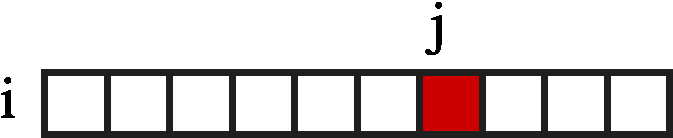
\includegraphics[width = 0.4\textwidth]{network_demand3}
\end{figure}
}
\only<3>{\vspace{0.12in}}
\begin{itemize}
\item<2-> Various factors (/topics) can affect the probability of location $j$ being the destination; e.g., locality, time, weather, etc.
\only<3>{
\begin{align*}
p(j) = &\text{importance(locality}|\text{location i)}\cdot p(j|\text{locality}) + \\
&\text{importance(time}|\text{location i)}\cdot p(j|\text{time}) + \\
&\cdots
\end{align*}
}
\item<4-> In general, the probability of location $j$ being the destination is:
\only<4->{
\begin{equation*}
p(j) = \sum_{k} p(k|i)\cdot p(j|k)
\end{equation*}
}
\item<5-> Our goal is to find the best $p(k|i)$ for every $i$ and $p(j|k)$ for every $k$ that matches the training data.
\end{itemize}
\only<6->{
\begin{textblock*}{11cm}(1cm,4.2cm)
\begin{alertblock}{}
We use the \textbf{log likelihood estimation} method with the \textbf{expectation maximization} algorithm to find the unknown probability distributions.
\end{alertblock}
\end{textblock*}
}
\end{frame}

\section{SPARP Mechanism}
\frame{\frametitle{Outline}\tableofcontents[currentsection]}

\begin{frame}\frametitle{Income \& Revenue}
Assuming $\rho_r$ is the platform's share of ride $r$:
\begin{align*}
payment(\pi_d, \hat{\theta_d}) &= \sum_{r \in \pi_d} \rho_r\\
income(\pi_d, \hat{\theta_d}) &= \sum_{r \in \pi_d} fare(r) - payment(\pi_d, \hat{\theta_d})
\end{align*}
\vspace{0.2in}
\only<2->{
therefore,
\begin{equation*}
revenue(M(\mathcal{D}, \mathcal{R})) = \sum_{d \in \mathcal{D}} payments(\pi_d, \hat{\theta_d})
\end{equation*}
}
\end{frame}

\begin{frame}\frametitle{Payments}
Ideally the framework should be:
\begin{itemize}
\item Budget Balanced; i.e., $revenue(M(\mathcal{D}, \mathcal{R}) \geq 0$
\only<2->{
\begin{exampleblock}{}
If for every request $r$, $\rho_r \geq 0$, the platform is budget balanced.
\end{exampleblock}
}
\item<3-> Individually Rational; i.e., $\forall d \in \mathcal{D} \quad u(\pi_d, \hat{\theta_d}, \theta_d) \geq 0$
\only<4->{
\begin{block}{}
If for every request $r$ assigned to driver $d$, $\rho_r \leq bid_d^r$, the platform is individually rational.
\end{block}
}
\item<5-> Truthful; i.e., $\forall d \in \mathcal{D} \ \forall \hat{\theta_d} \in \Theta \quad u(\pi_d, \hat{\theta_d}, \theta_d) \leq u(\pi_d, \theta_d, \theta_d)$
\only<6->{
\begin{alertblock}{}
If for every request $r$, $\rho_r$, is set to the second highest bid, the platform is truthful.
\end{alertblock}
}
\end{itemize}
\end{frame}

\begin{frame}\frametitle{Second-price Auction}
\only<1>{
\begin{figure}
	\centering
    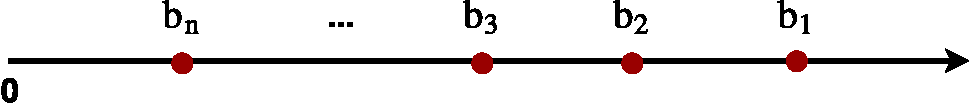
\includegraphics[width = 0.8\textwidth]{sparp1}
    \label{fig:quality}
\end{figure}
}
\only<2>{
\begin{figure}
	\centering
    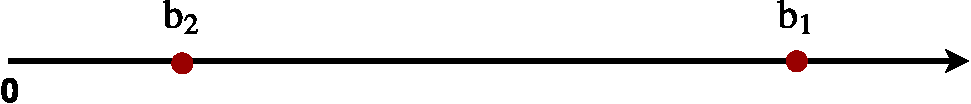
\includegraphics[width = 0.8\textwidth]{sparp2}
    \label{fig:quality}
\end{figure}
}
\only<3->{
\begin{figure}
	\centering
    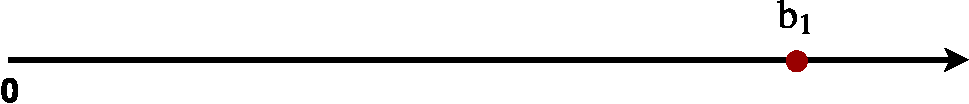
\includegraphics[width = 0.8\textwidth]{sparp3}
    \label{fig:quality}
\end{figure}
}
\begin{itemize}
\item In second-price auction, driver with $b_1$ wins but has to pay $b_2$ to the server.
\item<2-> Issues:
\begin{itemize}
\item<2-> What if $b_2$ is very small?
\item<3-> What if there is no $b_2$?
\end{itemize}
\end{itemize}
\end{frame}

\begin{frame}\frametitle{Reserved Price}
\begin{block}{}
$\forall r$, the reserved price $b_s^r$, is the minimum price the platform sets as the payment it expects. 
\end{block}
\begin{itemize}
\item<2-> If $b_s < b_2$: Driver with $b_1$ wins and pays $b_2$.
\item<3-> If $b_1 < b_s$: We assume $b_1$ wins and pays $b_2$.
\item<4-> If $b_2 < b_s < b_1$: Driver with $b_1$ wins and pays $b_s$.
\end{itemize}
\only<4->{
\begin{figure}
	\centering
    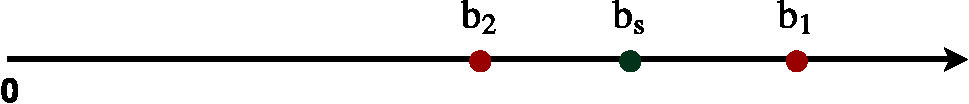
\includegraphics[width = 0.8\textwidth]{sparp4}
    \label{fig:quality}
\end{figure}
}
\only<2>{
\begin{figure}
	\centering
    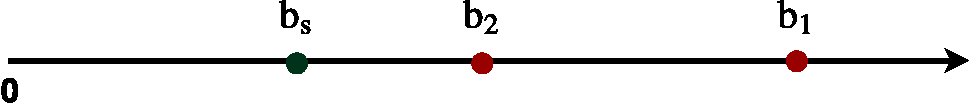
\includegraphics[width = 0.8\textwidth]{sparp5}
    \label{fig:quality}
\end{figure}
}
\only<3>{
\begin{figure}
	\centering
    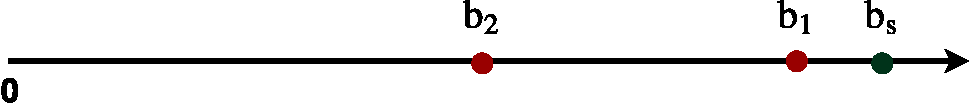
\includegraphics[width = 0.8\textwidth]{sparp6}
    \label{fig:quality}
\end{figure}
}
\begin{itemize}
\item<5-> We assume for every $r$:
\begin{equation*}
b_s^r = \text{base fare of }r - \text{cost of most expensive driver}
\end{equation*}
\end{itemize}
\end{frame}

\section{Experiments}
\frame{\frametitle{Outline}\tableofcontents[currentsection]}

\begin{frame}\frametitle{Setup}
\begin{itemize}
\item Data Set: New York City's Taxi data set
\only<1>{
\begin{itemize}
\item<1> 40K drivers \& 500K trips per day
\item<1> pickup/dropoff points, request time
\end{itemize}
}
\item<2-> Algorithms:
\only<2>{
\begin{itemize}
%\item Prediction Model
%\begin{itemize}
%\item LSTM
%\item LORE(Additive Markov Chains)[3]
%\end{itemize} 
%\item Revenue Generation
%\begin{itemize}
\item FPACB (First-price Auction w/ Competitive Bidding)[1]
\item SPA (Second-price Auction)
\item SPARP (Second-price Auction w/ Reserved Price)
%\end{itemize}
\end{itemize}
}
\item<3-> Parameters:
\only<3>{
%\vspace{-0.25in}
\begin{table}[!ht]
	\begin{center}
		\begin{tabular}{|c|c|}
			\hline
			Parameter & Values \\
			\hline \hline
%            Gide Size (km) & 1, \textbf{2}, 3, 4, 5 \\ 
%			\hline
%			Time Slot Size (hour) & 1, \textbf{2}, 3,  4, 5, 6\\ 
%			\hline
			\# of Drivers & 1000, 2000, \textbf{5000},  10000, 20000\\ 
			\hline
			Max Allowed Detour & 25\%, \textbf{50\%}, 75\%, 100\%\\
			\hline
		\end{tabular}
	\end{center}
\end{table}
}
\item<4-> Use the  Pricing Model in [1].
\end{itemize}
\only<2>{
\vspace{1.1in}
\tiny{[1] Asghari et. al., Price-aware Real-time Ride-sharing at Scale: An Auction-based Approach, SIGSPATIAL'17}
%\tiny{[3] Zhang et. al., Lore: Exploiting sequential influence for location recommendation, SIGIR'13}
}
\only<4>{
\vspace{1.6in}
\tiny{[1] Asghari et. al., Price-aware Real-time Ride-sharing at Scale: An Auction-based Approach, SIGSPATIAL'17}
}
\end{frame}

%\begin{frame}\frametitle{Prediction Model}
%\begin{itemize}
%\item Used k-fold cross validation to get train/test data
%\item Used the Kullback-Leibler Divergence(KLD) metric to evaluate the outcome of the model:
%\small{
%\begin{equation*}
%KLD\left(P \middle\| Q\right)=\sum_i P(i) \log \frac{P(i)}{Q(i)}
%\end{equation*}
%}
%\end{itemize}
%\vspace{-0.25in}
%\begin{figure}
%	\centering
%   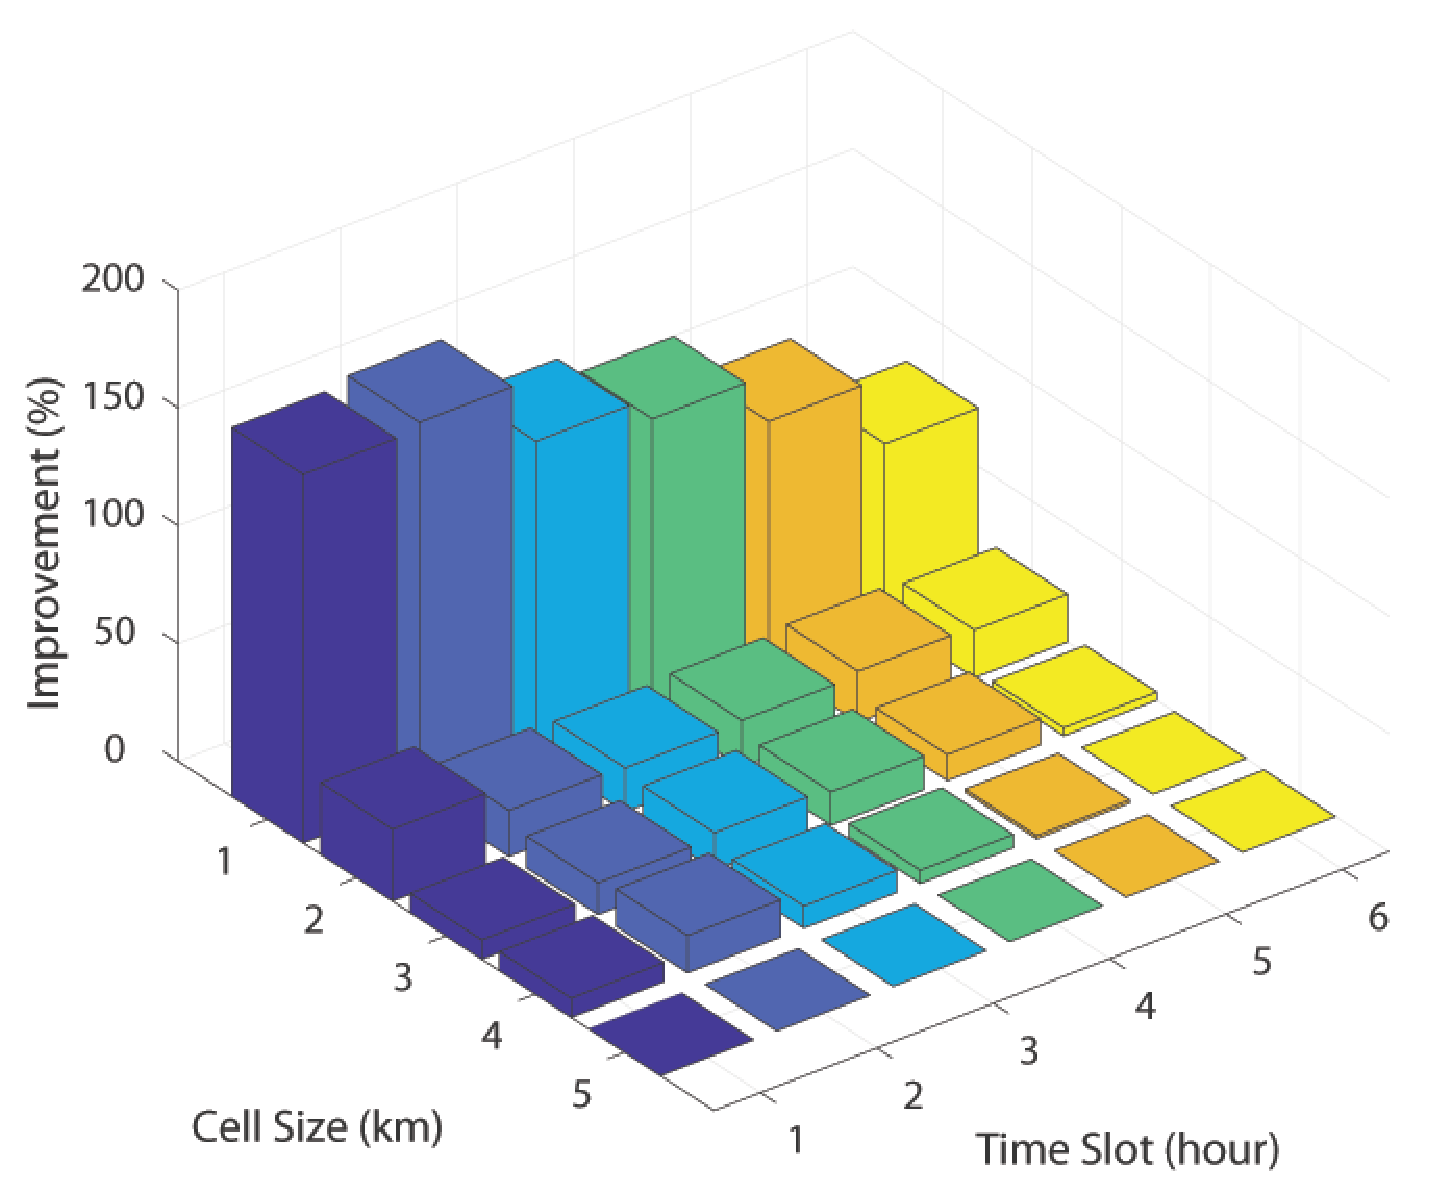
\includegraphics[width = 0.45\columnwidth]{klddiff}\\
%    \tiny{\textbf{\textit{LSTM Vs LORE - Varying Cell \& Time Slot}}}
%\end{figure}
%\end{frame}

\begin{frame}\frametitle{Untruthful Bidding}
\begin{itemize}
\item Use LSTM to predict the number of drivers
\item Assume the bids are uniformly distributed in $[0, \text{base fare of r}]$
\end{itemize}
\begin{table}
  \centering
  \begin{tabular}{|c|c|c|c|c|}
    \hline
    \multicolumn{2}{|>{\columncolor{kugray5}}c|}{}&\multicolumn{3}{c|}{Untruthful Drivers (\%)}\\
    \arrayrulecolor{kugray5}
    \arrayrulecolor{black}
    \cline{3-5}
    \multicolumn{2}{|>{\columncolor{kugray5}}c|}{}&25\%&50\%&75\%\\
    \hline \hline
    \multirow{4}{*}{\begin{turn}{90}Trutful\end{turn}} &Assigned Requests (Average)&14.33&14.19&13.04\\
    \cline{2-5}
                         		&Assigned Requests (Median)&8&\textcolor{blue}{6}&9\\
    \cline{2-5}
                         		&Income per Mile (Average)&\$1.00&\textcolor{red}{\$1.00}&\$1.00\\
    \cline{2-5}
                         		&Income per Mile (Median)&\$1.00&\$1.00&\$1.00\\
    \hline \hline
    \multirow{4}{*}{\begin{turn}{90}Untruthful\end{turn}}&Assigned Request (Average)&13.51&13.49&12.67\\
    \cline{2-5}
                         		&Assigned Requests (Median)&7&\textcolor{blue}{6}&8\\
    \cline{2-5}
                         		&Income per Mile (Average)&\$1.24&\textcolor{red}{\$1.25}&\$1.24\\
    \cline{2-5}
                         		&Income per Mile (Median)&\$1.21&\$1.23&\$1.23\\
    \hline
  \end{tabular}
  \label{tab:untruthful}
\end{table}
\end{frame}

\begin{frame}\frametitle{Revenue Generation}
\begin{itemize}
\item Compared the revenue of SPA \& SPARP w/ that of FPACB
\end{itemize}
\begin{columns}
\column{0.5\textwidth}
\begin{figure}
	\centering
    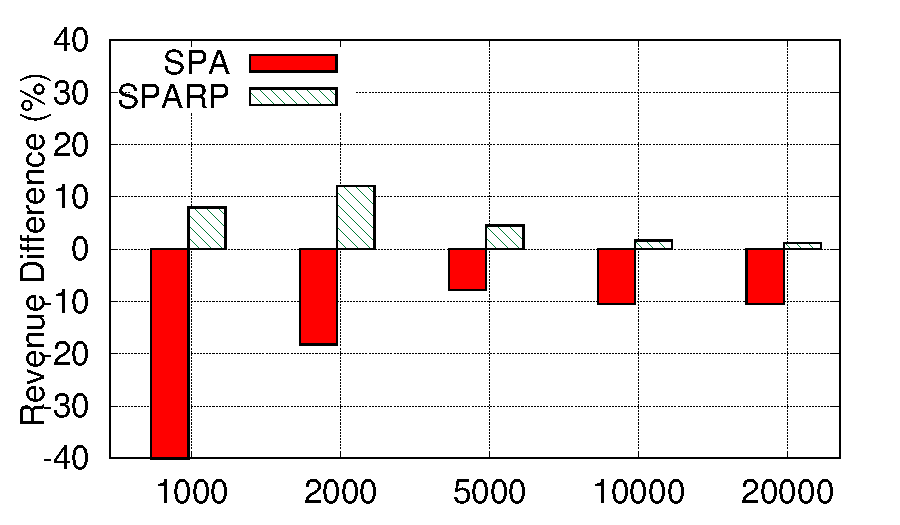
\includegraphics[width = 0.95\columnwidth]{nd2revdiff}\\
    \small{\textbf{\textit{Number of Drivers}}}
\end{figure}
\column{0.5\textwidth}
\begin{figure}
	\centering
    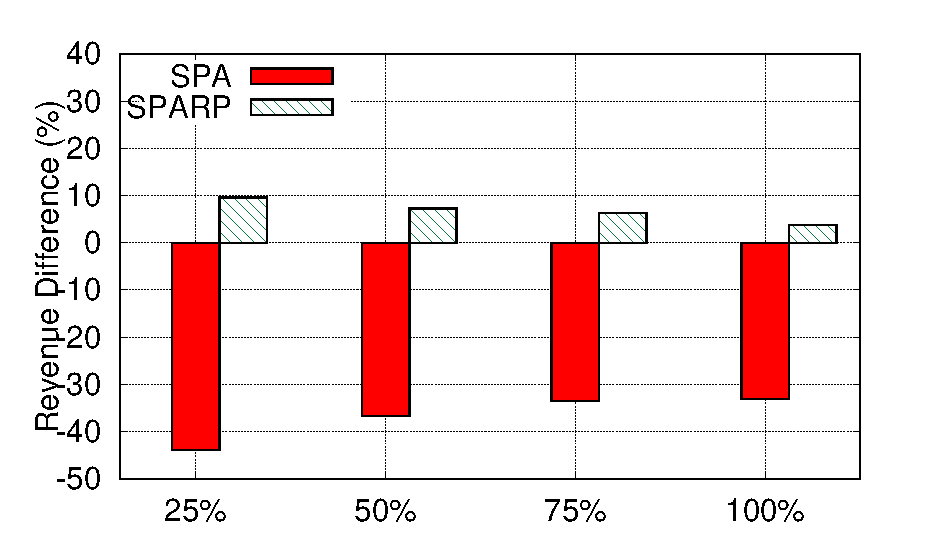
\includegraphics[width = 0.95\columnwidth]{mad2revdiff}\\
    \small{\textbf{\textit{Max Allowed Detour}}}
\end{figure}
\end{columns}
\end{frame}

\section*{Q \& A}
\begin{frame}\frametitle{Questions}
\begin{center}
	
\includegraphics[scale=0.3]{QandA.jpg}
\end{center}
\end{frame}




\end{document}